\chapter{Object reconstruction and identification}\label{chp:objects}

In CMS, physics objects such as electrons, muons, taus, photons, and hadrons 
can leave different signals in multiple detector components.
An illustration of how different particles interact with the CMS detector is shown in Figure~\ref{fig:cms_interact}.
As various particles are produced by $pp$ collisions in each event, 
the reconstruction of them requires a holistic processing of the information from all parts of the detector. 
This is achieved by the particle-flow (PF) algorithm~\cite{Sirunyan_2017}, which combines all detector signals per event
and finds the optimal identification and reconstruction of individual particles (PF candidates).
Properties of each PF candidate are calibrated centrally by CMS and provided to the analyzers.
The selection of each type of physics object is optimized by the analyzers based the characteristics of their analyses.

\begin{figure*}[!htb]
    \centering
    \captionsetup{justification=justified}
    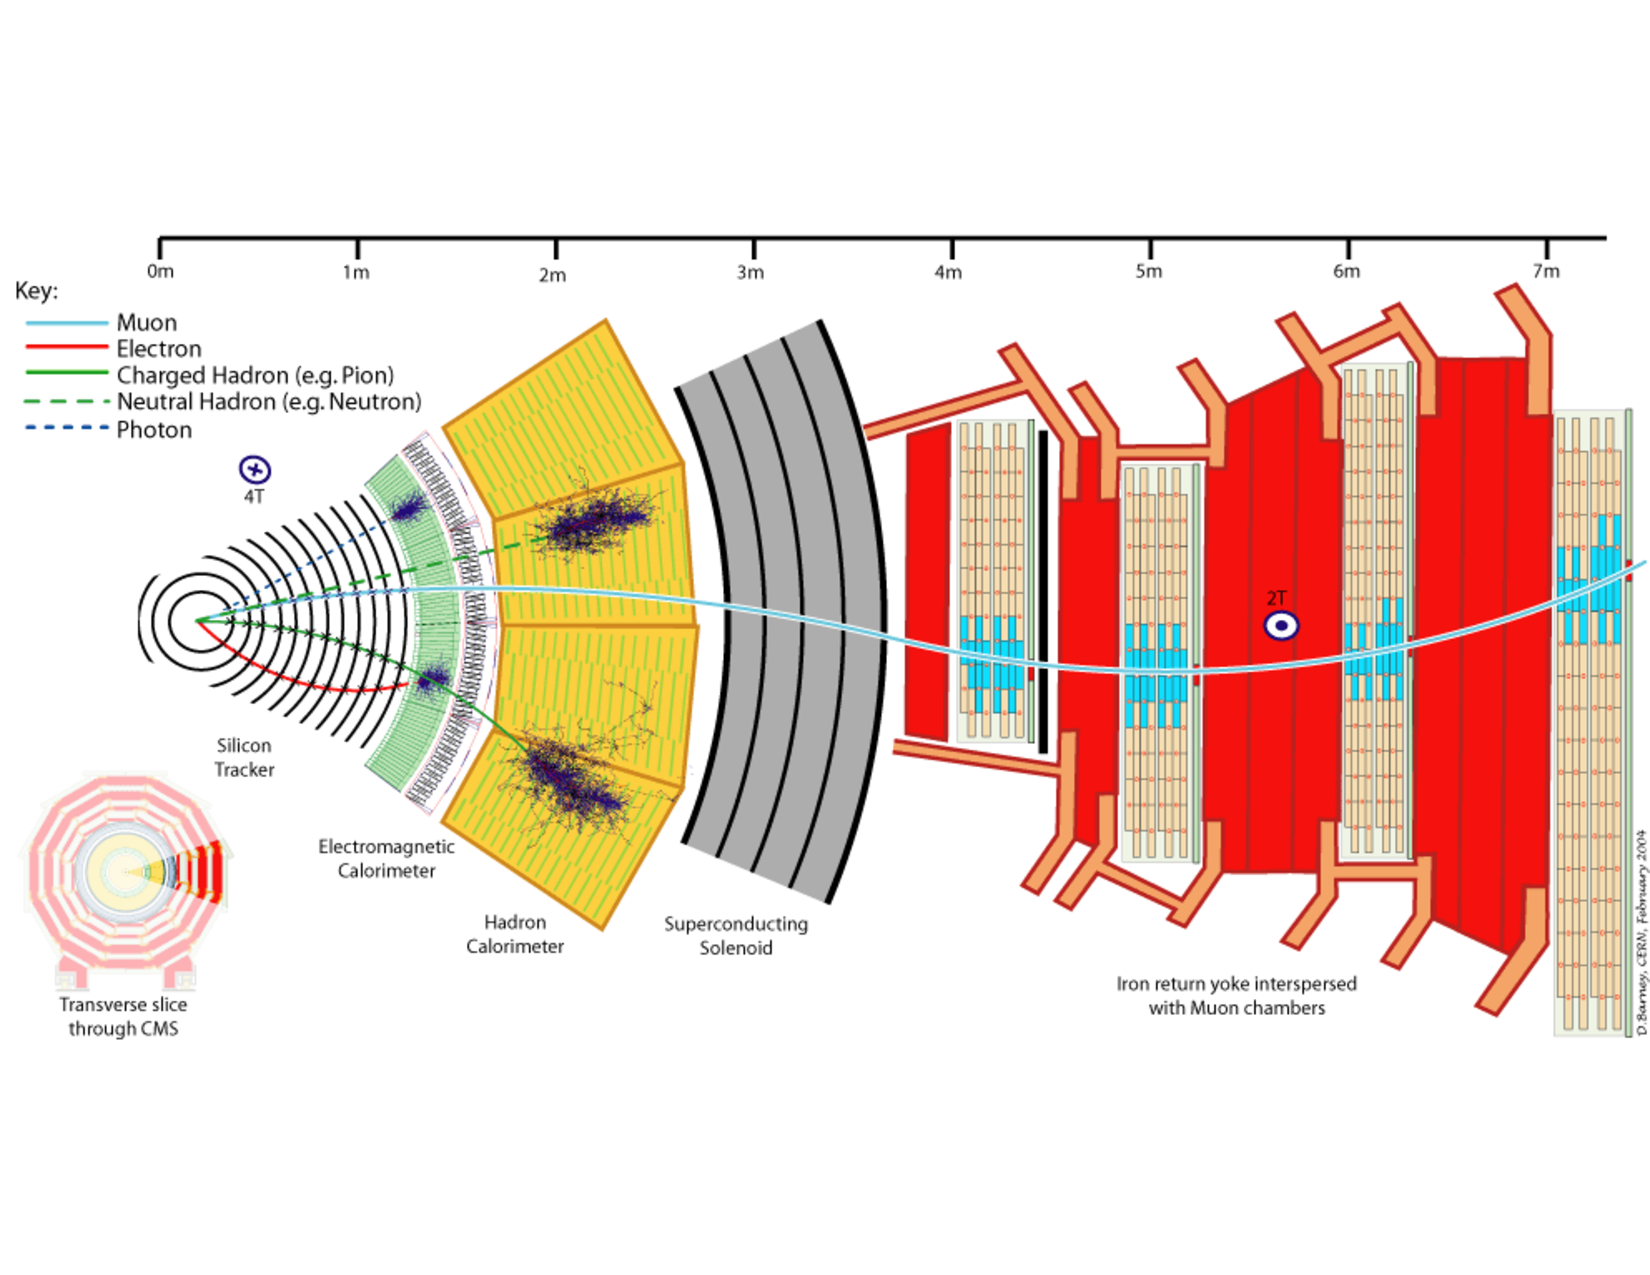
\includegraphics[width=0.98\textwidth]{pics/object_reco/CMS Slice.pdf}
    \caption{A transverse view of the CMS detector layout in the barrel region,
             with illustrations of the interactions between different particles and different detector components.
             Plot taken from Ref.~\cite{Davis:2205172}.}
    \label{fig:cms_interact}
\end{figure*}

Section~\ref{sec:obj_reco} gives a brief description of the reconstruction sequence for different particles.
Section~\ref{sec:obj_sel} lists the selection criteria for different objects adopted in the \hmm analysis.


\section{CMS object reconstruction}\label{sec:obj_reco}

In $pp$ collisions in CMS, final-state particles are produced at the beam interaction region. 
As they travel outward, they first enter the tracker system, in which the trajectories of charged particles 
(electrons, muons, and charged hadrons) bend in a strong uniform magnetic field and leave hits in the tracker layers. 
Passing the tracker, electrons and photons are absorbed in the ECAL, which in turn yields the measurements of their position and energy.
Hadrons may leave energy deposits in the ECAL as well, but can only be fully absorbed in the HCAL encircling the ECAL. 
Muons and neutrinos pass the calorimeters and the superconducting magnet with little or no interactions.
Muons then bend and leave hits in the muon detectors outside of the magnet, 
while neutrinos escape all detector layers without leaving any electronic signal.
A graphical summary of these interactions is given in Figure~\ref{fig:cms_interact}.

The PF algorithm combines all detector signals described above and attains a global determination of the final-state particles, 
along with the measurements of their properties.
Particles are identified and reconstructed in a sequential manner in PF and are described accordingly in the following sections:
tracks of charged particles are first build based on the tracker hits (Section~\ref{sec:reco_track}); 
vertices are reconstructed from groups of compatible tracks (Section~\ref{sec:reco_pv});
the interaction region is profiled by putting many vertices together (Section~\ref{sec:reco_bs});
muons and electrons are identified by associating tracks to signals in either the muon chambers or the ECAL (Section~\ref{sec:reco_muon} and ~\ref{sec:reco_ele});
hadrons and photons are reconstructed by combining measurements from ECAL, HCAL, with unmatched tracks (Section~\ref{sec:reco_phot} and~\ref{sec:reco_had});
muons, electrons, hadrons, and photons are all single final-state particles called PF candidates, 
which can be encapsulated as jets or hadronic decays of \tau leptons;
and finally, the missing transverse momentum (\MET) is defined as the negative of the vectorial sum of all PF candidates,
indicating the presence of neutrinos from the collision (Section~\ref{sec:reco_met}).

\subsection{Tracks}\label{sec:reco_track}

Tracks are the best measured objects in CMS and are the foundation of the reconstruction of various particles.
Any charged particle can leave hits in the tracking system and can be reconstructed as a track.
Tracks can later be linked to signals in the muons detectors and identified as a muon, 
or be linked to energy deposits in the ECAL and identified as an electron,
or be linked to energy deposits in the HCAL and identified as a charged hadron.
A ensemble of tracks can also provide information on the interaction vertices, 
opening the possibility to identify colliding point, converted photons, 
secondary decays of \Pqb quarks and \tau ~leptons, and unexpected long-lived particles (LLPs).

In a typical $pp$ event at CMS during the 2016-2018 data-taking period, 
where the center-of-mass energy is 13 \TeV and the pileup averages about 34,
order of a thousand tracks are produced by the collisions, leaving numerous hits in the tracking layers.
In order to correctly sew these hits into tracks, a track finder based on a combinatorial Kalman filter (KF)~\cite{Adam:934067} is applied:
\begin{itemize}
  \item Initial seeds are generated with a few hits compatible with a charged particle trajectory.
  \item For each seed trajectory, the next layer is surveyed for hits compatible with the seed.
        A new trajectory candidate is generated for each possible new hit association, 
        with the trajectory quality updated based on the compatibility.
  \item This pattern recognition is repeated until it reaches the outermost layer.
        The total number of trajectory candidates is truncated at each layer to avoid an exponential increase. 
  \item The final trajectory candidates are cleaned for duplications, 
        and are evaluated for their properties.
\end{itemize}

The KF track finder is applied in several successive iterations~\cite{Collaboration_2014}, 
each targeting a different type of track: first prompt high \pt tracks, then prompt low \pt tracks,
followed by displaced tracks, and finally tracks with significant detector inefficiencies.
After each iteration, all hits associated with the selected tracks are removed from the consideration of the remaining iterations.
In this way, the tracking efficiency is maximized while the mis-reconstruction rate is kept as low as possible.

Tracks identified by the finder algorithm are refit with a Kalman filter and smoother to evaluate their properties:
transverse momentum, direction, and origin.
A Kalman filter starts with the innermost hits (typically four) on the track, 
and builds the covariance matrix~\cite{Strandlie:927379}, 
which is used to propagate hit uncertainties into the uncertainties of global track properties. 
This filter proceeds forward through the full list of hits, 
updating the trajectory estimate and the covariance matrix with each hit.
The hit position uncertainty is re-evaluated using the current trajectory estimate as well at each step. 
As a complement, an additional filter is initialized at each hit with the result of the forward filter 
but works backward using all hits outside of the current hit. 
The weighted average of the track parameters from the two filters is taken as the estimate of the trajectory at that hit.
This practice is called a smoothing procedure which ensures the optimal estimate at any hit on the track
including, in particular, the innermost and outermost hit.
The track is extrapolated to the interaction region and to the calorimeters and muon chambers from the closest hit (the innermost or outermost hit),
which are specially important for vertex reconstruction and for track matching to signals in other detectors, respectively.


\subsection{Primary vertices}\label{sec:reco_pv}

In $pp$ collisions at the LHC, multiple $pp$ interactions can happen in the same bunch crossing, known as pileup.
Most of them produce tracks, while only a tiny fraction of the interactions are hard scatters interesting to physicists.
All the $pp$ interactions happen in the beam interaction region (called the beam spot) which spreads along the beam axis,
following a normal distribution with a standard deviation of a few centimeters.
In order to separate different tracks belonging to different interactions, 
tracks are extrapolated to the beam axis to find their origins (vertices).
The vertex reconstruction is performed with the follow procedure~\cite{Collaboration_2014}:
\begin{itemize}
\item Tracks are first selected by the requirement on their compatibility with the center of the beam spot, 
      along with some track quality criteria.
      This selection picks out tracks from secondary decays and tracks with low quality, 
      ensuring a high reconstruction efficiency. 
\item Tracks are then clustered based on their z-coordinates at their point of closest approach to the center of the beam spot.
      The clustering algorithm starts with a large series of hypothetical vertices along the beam axis, 
      and optimize the global assignment based on the likelihood of each track associated to each hypothetical vertex.
      After the optimization, a few ensembles of hypothetical vertices emerge, each considered as a vertex candidate.
\item The position of each vertex candidate is fit with the parameters of all the tracks associated to it.
      The fit is performed adaptively with a weight assigned to each track reflecting the likelihood that it genuinely belongs to the vertex.
      The weights are updated in each iteration until the sum of weights is maximized. 
\end{itemize}

All the resulting vertices along the beam axis are called the primary vertices (PVs).
The PVs are ordered by the quadratic sum of the \pt of their tracks, $\sum \pt^{2}$,
and the PV with the highest $\sum \pt^{2}$ is considered as the hard-scatter vertex, 
while the other vertices are considered as pileup vertices.
In most physics analyses, the hard scatter vertex is the interaction of interest,
and is therefore sometimes referred to as the single primary vertex.


\subsection{Beam spot}\label{sec:reco_bs}
The beam spot refers to the 3D-region in which $pp$ collisions happen, 
and is determined from the distribution of primary vertices from many events.
The position and size of the beam spot are evaluated as the x, y, z coordinates 
of the beam spot center and their corresponding standard deviations.
These values are determined per luminosity section, which is a period of 23 seconds of event collection.
If no significant shift of the beam spot center is observed in multiple consecutive luminosity sections,
their beam spot position values are merged to extract a final estimate.
The beam emittance grows with time, leading to a gradual growth of beam spot size.
Therefore the beam spot size values are kept per luminosity section instead of merging multiple ones. 

\subsection{Muons}\label{sec:reco_muon}

The muon detectors in CMS allows muons to be identified with high efficiency,
which is guaranteed by the upstream calorimeters absorbing other particles (except neutrinos).
The muon reconstruction combines information from both the tracker and muon chambers, 
building three different reconstructed muon types~\cite{Sirunyan_2018}:
\begin{itemize}
      \item \textit{Standalone muon.} 
            Hits in muon chambers are clustered into track segments with a KF track finding procedure
            similar to the one applied in track reconstruction in Section~\ref{sec:reco_track}.
            Track segments are built with DT or CSC hits as seeds and are grown into trajectories containing DT, CSC, and RPC hits. 
            The resulting tracks are called the standalone muon tracks.
      \item \textit{Tracker muon.}
            Each track built with tracker hits in Section~\ref{sec:reco_track} with a \pt larger than 0.5 ~\GeV 
            and a total momentum $p$ larger than 2.5 \GeV is extrapolated to the muon system.
            A comparison is made between the spatial coordinates of the extrapolated tracker track and the nearby DT or CSC muon segments.
            If the extrapolated track matches at least one muon segment,
            the tracker track is considered as a tracker muon track.
      \item \textit{Global muon.}
            A global muon is build starting with a standalone muon and matched to a tracker track.
            The matching is performed by comparing KF parameters of the two tracks.
            A combined fit is performed using information from both the tracker track and the standalone muon track
            to determine the final parameters of the global muon track. 
\end{itemize}

Most tracker muons are also global muons, as most muons can be successfully reconstructed as standalone muons.
The track muons are more efficient in identifying low \pt muons, 
which may only leave hits in the innermost muon station but are not energetic enough to reach the others,
failing to be reconstructed as a global muon.
This higher efficiency, on the other hand, is accompanied with a higher misidentification rate,
as hadron shower remnants can sometimes reach the innermost muon station, known as the punch-through,
which could fake a tracker muon but not a global one. 

The momentum of each global muon is measured fitting all tracker hits plus either zero or one, or multiple hits in muon detectors,
depending on their compatibility with the extrapolated tracker track.
Since the tracker hits have better spatial resolution than the muon detector hits, 
the contribution from muon detectors is marginal for muons with \pt $<$ 200 \GeV.
On the other hand, for muons with \pt $>$ 200 \GeV, the information from muon detectors improves the measurement significantly,
because the tracks of these high \pt muons are very straight, and muon detector hits, being far from the tracker hits,
provides essential information for the track curvature evaluation.

The isolation is another important property of muon tracks.
It help to distinguish between muons from energetic prompt interactions (prompt muons) and the ones from weak decays within jets (non-prompt muons). 
It is defined as the ratio to the muon \pt by the sum of energy in a geometric cone, 
$\Delta{}R = \sqrt{(\Delta{}\phi)^{2} + (\Delta{}\eta)^{2}}$.
The summation considers all charged hadrons and neutral particles in PF~\cite{Sirunyan_2017},
\begin{equation}\label{eq:iso_def}
    I_{\text{PF}} = \sum_{h^{\pm}, HS} \pt^{h^{\pm}} + \text{max}(0, \sum_{h^{0}} \pt^{h^{0}} + \sum_{\gamma} \pt^{\gamma} - \Delta\beta \sum_{h^{\pm}, PU} \pt^{h^{\pm}})
\end{equation}
where HS means hard scatter and PU means pileup.
$h^{0}$ and $h^{\pm}$ in the equation are neutral and charged hadrons.
This calculation aims to mitigate the contamination from pileup and only focus on the hard scatter.
The factor $\Delta\beta$ is set to be 0.5, which corresponds approximately to the ratio of neutral particle to charged hadron production 
in inelastic $pp$ collisions, as an estimate to remove the pileup particle energy. 

In addition to the kinematic variables, a set of variables is defined to reflect the quality of the muon reconstruction,
such as the $\chi^{2}$ of the track fit, the number of hits per track (either in the tracker or the muon detectors, or both), 
and for global muons specifically, the degree of matching between the tracker track and the standalone muon track.
There are other variables evaluating whether the muon track is compatible with the primary vertex, 
and whether a kink can be found in the muon track.
Based on these variables, CMS offers several sets of official muon identification criteria for physics analyses,
each targeting a different type of muon.
The specific muon selection criteria adopted in the \hmm analysis is detailed in Section~\ref{sec:sel_muon}.


\subsection{Electrons}\label{sec:reco_ele}

Electrons (and positrons) produce hits in the tracker layers and are eventually absorbed by the ECAL.
Both the tracker and ECAL provide information on electron identification but both suffer from significant inefficiencies:
most electrons emit bremsstrahlung photons as they travel through the tracker layers and lose a sizeable fraction of their energy,
which degrades the quality of the reconstructed tracks and biases the momentum measurements;
while most of the electron energy including the bremsstrahlung photons is captured by a series of neighboring ECAL units,
this energy deposit is very often overlapped with deposits from other photons and hadrons and is very hard to disentangle.
The electron identification relies on the combination of tracker and ECAL information, starting with two types of seed~\cite{cmscollaboration2020electron}:
\begin{itemize}
    \item \textit{ECAL-based seed.}
          Energy deposits in several ECAL channels are grouped into clusters. 
          If the energy deposit in a cluster exceeds 1 \GeV, 
          it is considered as a potential incident particle and the cluster is called a seed cluster.
          Since a final state electron may reach the ECAL as several electrons and/or photons 
          due to bremsstrahlung radiation and photon conversion, which scatter in multiple clusters tangent to the electron track,
          clusters near the seed cluster are further grouped into a supercluster (SC).
          A SC is defined with a small window in \eta{} and an extended window in \phi{} 
          in order to follow the azimuthal bending of electron tracks in the magnetic field.
          If a SC can be loosely matched to a track seed (as described in Section~\ref{sec:reco_track}),
          and if there is no significant energy deposit in the HCAL towers behind the SC,
          this SC along with the track seed(s) linked to it are selected as an ECAL-based electron seed.

    \item \textit{Track-based seed.}
          An electron seed can also be built from a generic track if its \pt exceeds 2 \GeV.
          When the energy radiated by the electron is small, the reconstructed track has good quality 
          and can be extrapolated to the ECAL surface.
          If the ratio of the closest ECAL cluster energy to the track momentum is compatible with unity,
          The track along with the ECAL cluster is selected as a track-based seed.
          For electrons that lose considerable energy via photon emission, 
          their tracks may have kinks and generally have unideal qualities.
          These tracks are selected with some loose quality criteria and refit with a Gaussian-sum filter (GSF),
          which is more CPU intensive than the KF used for general tracking,
          but more adapted to sudden and substantial energy losses along the trajectory.
          The GSF refit track is extrapolated to the ECAL surface, 
          and a multivariate discriminator is evaluated combining the track and ECAL information.
          The track and the ECAL cluster is considered as an electron seed if the discriminator suggests so. 

\end{itemize}

Electron seeds obtained from these two approaches are merged and submitted to a more exhaustive GSF refit.
In addition, a survey is performed among generic tracks near the seeds, 
to pick up any track pair with a common displaced vertex.
Such track pairs are likely to originate from photon conversions (more details in Section~\ref{sec:reco_phot}).
Conversion tracks made lead to a refinement of the SC shape and an update (or removal) of the GSF tracks.
A electron is reconstructed only if the GSF track can be built, 
and if the HCAL energy deposit behind the ECAL SC does not exceed 10\% of the SC energy.
Energy collected by the ECAL SC is subject to losses for several reasons:
material in the tracker, electromagnetic shower leakages, and intermodule gaps in ECAL.
The total energy in the ECAL SC is corrected with a multivariate regression algorithm to account for these energy losses.
The final energy assignment for electrons is based on a combination of 
the corrected SC energy and the momentum of the GSF track.

The electron identification is based on several aspects of the reconstruction.
The isolation of electrons follows the definition in Equation~\ref{eq:iso_def} 
and is the main handle to distinguish prompt electrons from non-prompt ones.
The electromagnetic show shape also helps to reject fake electrons from hadrons 
and is described by a few variables: 
the ratio between the SC energy and the HCAL energy behind it,
the variable $\sigma_{i\eta{}i\eta}$ indicating the second moment of the ECAL energy in a $5 \times 5$ crystal array,
and the variable $R_{9}$ defined as the most energetic $3 \times 3$ crystal array divided by the total SC energy.
A few other variables evaluates the compatibility between the ECAL SC and the track:
the distance in $\eta$ between the seed cluster and the track,
the distance in $\phi$ between the energy-weighted SC position and the track,
the difference between the inverse of the SC energy and the inverse of the track momentum. 
Furthermore, some other variables are also included accounting for how many missing hits are in the track 
and whether the electron is likely to come from the conversion of a photon.

CMS offers several sets of official electron identification criteria based on these variables,
either in a cut-based fashion or as a multivariate discriminator.
The specific electron selection criteria adopted in the \hmm analysis is detailed in Section~\ref{sec:reco_ele}. 

\subsection{Photons}\label{sec:reco_phot}

Photons can be produced by various processes in CMS: from prompt interactions, 
from bremsstrahlung emission of electrons, and from secondary decay of hadrons (mostly $\pi^{0}$).
Although photons themselves do not produce hits in trackers, 
they have a significant probability to convert into an electron-positron pair in the tracker material.
Photons, if not converted, are all fully absorbed by the ECAL,
whose signals can very often be mixed with the signals from nearby electrons and hadrons if there are any.
As a result, photon identification is entangled with the reconstruction of electrons and hadrons.
In CMS, photons can be defined in three cases at different stages of the PF reconstruction:
the converted photons based on displaced track pairs and their associated ECAL clusters,
the isolated unconverted photons based on ECAL deposits with little HCAL energy deposit behind it,
and the non-isolated unconverted photons based on ECAL deposits with significant HCAL energy deposit behind it.

The reconstruction of converted photons involves tracks and ECAL clusters, 
and is performed along with the reconstruction of electrons and isolated unconverted photons.
After the electron seeding stage, a conversion finding algorithm~\cite{2015photon} examines all tracks near the ECAL SC
and looks for tracks significantly displaced from the primary vertex.
If displaced tracks of different charges are found, they are paired with some proximity requirement 
and fit to a common vertex with a kinematic vertex fit.
These track-pair candidates are defined as converted photons if they satisfy thresholds on the quality of kinematic fit,
on the total \pt, and on the compatibility between the converted tracks and the associated ECAL clusters.

The reconstruction of isolated photons shares the same procedure as the electron reconstruction described in Section~\ref{sec:reco_ele},
and is only different at the last stage:
an electron is defined if a GSF track can be built from the seed, 
while a photon is defined if no GSF track can be built associated to the ECAL SC 
and if the \ET is greater than 10 \GeV.
These photon candidates from ECAL seeding are further retained if they are isolated from other tracks and ECAL clusters
and if there are no significant HCAL energy deposits around.
The corrected ECAL SC energy is used for the final photon energy assignment. 

More often, photons in CMS are produced by decays of hadrons 
and are not isolated from other calorimeter deposits.
The reconstruction of non-isolated photons is performed along with the reconstruction of hadrons, 
which is detailed in Section~\ref{sec:reco_had}.
Once muons, electrons, isolated photons, and charged hadrons are reconstructed by PF, 
the tracks and calorimeter deposits associated to them are masked,
leaving only unassigned ECAL and HCAL clusters.
In general, photons carry about 25\% of the total jet energy, all absorbed by the ECAL,
while neutral hadrons leave only 3\% of the total jet energy in the ECAL.
Therefore, within the tracker acceptance ($|\eta| < 2.5$), as charged hadrons are already identified,
all the unassigned ECAL deposits are considered as photons and all remaining HCAL deposits are considered as neutral hadrons.  
However, out of the tracker acceptance, charged hadrons cannot be distinguished from neutral ones.
Charged and neutral hadrons together leaves about 25\% of the total jet energy in the ECAL,
which is at the same level of photon energy.
ECAl deposits can no longer be assumed as photons.
In this case, hadrons are reconstructed with HCAL clusters, 
and a fraction of energy is removed from the associated ECAL clusters.
The remaining net ECAL clusters are reconstructed as photons.
The energy estimate of these non-isolated photons takes the uncorrected ECAL cluster energy. 

The identification of photons is based on the isolation and electromagnetic shower shape variables as described for electron identification (Section~\ref{sec:reco_ele}).
CMS offers identification criteria either as cut-based selections or a multivariate discriminator.
These identifications target only isolated photons, while the non-isolated one are encapsulated in jets (Section~\ref{sec:reco_had}).
Photons are not used in the \hmm analysis as primary physics objects, but are only used for the recovery of the energy losses in final state radiation (FSR).
The selection for FSR photons is described in Section~\ref{sec:fsr}. 

\subsection{Hadrons}\label{sec:reco_had}

Hadrons are produced in plenty by $pp$ collisions in CMS.
Charged hadrons leave hits in the tracker and all hadrons are fully absorbed by the calorimeters.
All hadrons are initiated by gluons or quarks in QCD process, and are always produced as cascades, known as jets.
As a result, their detector signals, especially in calorimeters, always overlap with one another.
As the detectors only provide information on the trajectory (for charged hadrons only) and energy of the hadrons,
CMS reconstruct hadrons as charged and neutral ones without further distinguishment of their exact composition.

Energy deposits in HCAL are grouped into clusters in a similar fashion as that in the ECAL seeding.
Cluster seeds are first identified as HCAL cells that have an energy over a threshold and larger than their neighboring cells.
Seeds are grown into topological clusters by iteratively including adjacent cells with an energy above another threshold.
A topological cluster may cover many seeds if they are connected by cells with significant energy deposits.
Each topological cluster is fit with a Gaussian-mixture model in which the energy distribution in the cells is assumed to be 
the sum of $N$ Gaussian energy distributions, where $N$ is the number of seeds in the topological cluster.
Each resulting Gaussian component is considered a a cluster.

Within the tracker acceptance, HCAL clusters linked to tracks are reconstructed as charged hadrons. 
Non-isolated photons and neutral hadrons are reconstructed from the remaining ECAL and HCAL clusters respectively.
Beyond the tracker acceptance, hadrons are reconstructed from the HCAL clusters without differentiating their charges,
and photons are reconstructed with the remaining ECAL clusters.

All hadrons (and non-isolated photons) are considered as PF candidates but are not used as individual physics objects for analyses.
PF candidates are clustered into more complex objects like jets and the hadronic decays of \tau{} leptons,
which are used in physics analyses indicating outgoing partons or \tau{} leptons from the collisions.  
Reconstruction of jets and hadronic \tau{} decays are detailed in Section~\ref{sec:reco_jet} and~\ref{sec:reco_tau}.


\subsection{Jets}\label{sec:reco_jet}

All partons carry color charges. 
They cannot exist as free particles because QCD forbids isolated color charges, known as color confinement.
When partons are emitted from collisions, the strong interaction potential grows rapidly between the color charges as they move away from each other.
Once the potential reaches a threshold known as Hagedorn temperature, corresponding to an energy of roughly 150 \MeV,
the excessive energy is converted into the production of a quark-antiquark pair in between the outgoing color charges. 
If the original outgoing partons are energetic enough, this process is repeated, leading to a cascade of quarks and gluons.
These quarks and gluons bind with each other and form hadrons which are color-neutral, known as the hadronization process.
Some of the hadrons have short lifetime and decay into photons, leptons, or lighter hadrons.
As a result, a parton produced in collisions are always received as a cluster of mixed particles that traverse with roughly collinear directions, known as a jet.
In $pp$ collisions at the LHC, on average, 65\% of the jet energy is carried by charged hadrons, 25\% by photons, and 10\% by neutral hadrons.

In particle-flow, jets are reconstructed with the anti-$k_{T}$ algorithm~\cite{Cacciari_2008, fastjet},
which clusters particles based on a parametrized distance between them.
Jet can be reconstructed considering all PF candidates (PF jets), 
or be reconstructed with PF candidate except charged hadrons from pileup vertices via charged hadron subtraction (CHS). 
The jet momentum is calculated as the vector sum of all of its constituent PF candidates, 
In the same fashion, an invariant mass of the jet is also calculated. 
PF jets are studied down to a \pt of 15 \GeV.

The energies of PF jets are systematically underestimated for several reasons.
Very low \pt charged hadrons loop in the tracker and do not reach the calorimeter.
It is usually difficult to cluster these tracks with other particles and many of them end up unassigned.
Neutral hadrons with low energy ($< 10 \GeV$) may not be successfully identified from the HCAL noise, and are sometimes not reconstructed.
Furthermore, neutral hadrons usually also leave energy deposits in the ECAL, 
which are systematically identified as (non-isolated) photons,
following the reconstruction procedure described in Section~\ref{sec:reco_phot}.
These ECAL deposits are calibrated following the photon hypothesis, 
which is not suitable for hadrons and leads to an systematic underestimate of energy.

To mitigate this systematic bias in the jet energy estimate, 
a jet energy correction (JEC) procedure~\cite{Khachatryan_2017} is applied,
which brings the jet response, defined as the mean ratio between the reconstructed jet energy to the true jet energy,
to unity across different \pt and $\eta$ regions.
The jet energy resolution is mostly determined by the resolution of the HCAL, 
therefore the relative resolution is better for more energetic jets.
After the JEC, in the barrel region, the relative energy resolution is typically 15\% for 20~\GeV jets,
10\% for 100~\GeV jets, and 5\% for 1~\TeV jets. 

The \hmm analysis uses PF+CHS jets, with JEC applied.
Jets are particularly important in the \qqH category which is tagged with two energetic forward jets.
In the \VH category, on the other hand, jets are not used explicitly but only considered for the calculation of the missing transverse energy. 
The selection criteria of jets are detailed in Section~\ref{sec:sel_jet}.

\subsection{B-jets}\label{sec:reco_btag}

Jets originating from bottom or charm quarks contain heavy-flavor hadrons, and are called heavy-flavor jets.
These heavy-flavor hadrons have lifetimes of the order of 1~ps, and their decays give rise to secondary vertices (SV) a few \mm away from the corresponding primary vertex. 
Therefore the heavy-flavor jets can be distinguished from the light-flavor ones (originating from light-flavor quarks or gluons).
The identification of jets initiated by \Pqb~quarks, called b-jets, are particularly important to both SM measurements and BSM searches.
CMS provides several algorithms to evaluate the probability of a jet to be a b-jet~\cite{Sirunyan:2017ezt}, among which the DeepCSV tagger is adopted in the \hmm analysis.

The DeepCSV considers many discriminating variables of a jet: the track multiplicity, the kinematic properties of the tracks in the jet,
the energy ratio and spatial separation between different tracks, the position and the invariant mass of secondary vertices, 
and the presence/absence of semileptonic decays of hadrons in the jet.
These variables are processed with a deep neural network, whose outputs are probabilities of the jet to contain one b hadron ($P$(b)), or two b hadrons ($P$(bb)),
or one c hadron ($P$(c)), or two c hadrons ($P$(cc)), or none of them ($P$(udsg)).  
The result $P$(b)~+~$P$(bb) is used as the figure-of-merit to set standard b-tagging working points in CMS.
Three working points are officially provided: the loose, medium, and tight tags, 
which are chosen with a misidentification rate of 10\%, 1\%, and 0.1\%, 
and correspond to a tagging efficiency of about 85-90\%, 70-75\%, and 50-55\%, respectively.
B-tagging relies heavily on the tracking information and is therefore only developed and applied inside the tracker acceptance region $|\eta| < 2.5$.

B-tagging are used in the \hmm analysis to identify the b-jets from the top quark decays in \ttH events, 
or to veto such decays in other event categories.
The exact criteria for b-tagged jet selection in the \hmm analysis is detailed in Section~\ref{sec:sel_jet}.

\subsection{Hadronic tau decays}\label{sec:reco_tau}

The \tau{} lepton has a mean lifetime of 0.3~ps and decays to either an electron or a muon plus two neutrinos, or a few hadrons plus one neutrino.
The reconstruction of leptonic \tau{} decays is unrealistic as they are only received by the detector as an electron or muon, 
which is hardly distinguishable from electrons or muons produced in other processes.
On the other hand, the reconstruction of hadronic \tau{} decays, denoted as $\tau_{h}$, can be achieved based on the track multiplicity, collimation, and isolation of the decay products.  

The main hadronic \tau{} decay modes contain either one or three charged hadrons, from zero to two neutral hadrons ($\pi_{0}$), and a neutrino.
Their detector signature resembles that of low-multiplicity jets.
Therefore in PF, $\tau_{h}$ candidates are reconstructed starting with PF jets as seeds. 
The reconstruction algorithm is called the hadrons-plus-strips (HPS) algorithm~\cite{tau2016, tau2018},
which picks charged hadrons from the seeding jet, and clusters photon and electron constituents of the seeding jet into "strips" in the $\eta-\phi$ plane.
Each strip is considered as a $\pi_{0} \to \gamma\gamma$ candidate inside the $\tau_{h}$ decay.
Different combinations of one or three charged hadron candidates plus up to two strips are tested for several $\tau_{h}$ hypotheses:
$\tau^{\pm} \to h^{\pm}h^{\mp}h^{\pm}\nu_{\tau}$, $\tau^{\pm} \to h^{\pm}\pi_{0}\pi_{0}\nu_{\tau}$,
$\tau^{\pm} \to h^{\pm}\pi_{0}\nu_{\tau}$, and $\tau^{\pm} \to h^{\pm}\nu_{\tau}$.
Hypotheses are rejected if they fail requirements on the invariant mass, the sum of charge, the isolation, and the track vertexing in cases of multiple tracks.
If multiple combinations inside a jet are compatible with the $\tau_{h}$ hypotheses, the one with the largest \pt is retained and all others are discarded.

The identification of $\tau_{h}$ candidates is performed separately against jets, electrons, and muons.
The ID discriminants can either be cut-based or MVA-based, on various kinematic properties of the $\tau_{h}$ candidates.
Several working points are provided for each discriminant, whose efficiencies range from 30\% to 70\% (vs jets), from 70\% to 90\% (vs electrons), and from 98\% to 99\% (vs muons),
all with a misidentification rate below 1\%.

Hadronic \tau{} candidates are not considered in the \hmm analysis.

\subsection{Missing transverse momentum}\label{sec:reco_met}

Neutral particles produced in $pp$ collisions that interact weakly with regular material can traverse the CMS detector undetected.
There is no way to determine their number, type, or exact direction.
However, when these particles are produced along with detectable particles: muons, electrons, photons, hadrons etc.,
their presence can be inferred from the detected particles as an imbalance in the total momentum perpendicular to the beam pipe.
This imbalance is referred to as the missing transverse momentum ($\vec{p}^{miss}_{T}$) or the missing transverse energy (\MET).
In practice, no distinguishment is made between \MET and the magnitude of the missing transverse momentum ($p^{miss}_{T}$) 
as there is no way to infer the invariant mass of the missing particle(s).

\MET itself is not a physics object but is crucial to physics analyses, 
both in SM measurements containing leptonic decays of the \PW boson
and in searches for new weakly-interactive particles beyond the SM.
CMS offers two ways to reconstruct the \MET~\cite{Sirunyan_2019}.
The PF \MET~\cite{collaboration_2015} is defined as the negative of the vector \pt sum of all PF candidates in the event.
The other reconstruction method is called the "pileup per particle identification" (PUPPI)~\cite{Bertolini2014},
which sums all PF candidates while rescaling the energy of all hadrons based on their likelihood of originating from the PV.
The PF \MET is used in the \hmm analysis.

In addition, another missing energy estimate based on high level physics objects, \MHT, are adopted in many analysis.
It sums only identified leptons and jets, instead of all PF candidates, 
in order to focus on the expected products of the prompt interaction.
In the \hmm analysis, the \MHT definition only considered leptons and jets that pass their selection criteria specific in~\ref{sec:obj_sel}. 

By its nature, the resolution of \MET (or \MHT) is much worse than other physics objects.
A mismeasurement on \MET can originate from proton debris falling out of the detector acceptance,
mis-reconstruction of objects and mis-association between pileup and primary vertices,
and in general experimental resolution in all detector components.
Improving the \MET estimate is the key to improve the precision of many measurements and the sensitivity of many searches.


\section{Object selection in the H to muons analysis}\label{sec:obj_sel}

\subsection{Muon selection}\label{sec:sel_muon}

CMS provides official muon identification (ID) criteria based on several kinematic variables:
the number of hits in the muon track; the fit quality of the muon track; 
the compatibility between the tracker track and the standalone muon for global muons;
and the compatibility between the muon track and the primary vertex.
The global track fit $\chi^{2}$ and a kink-finder $\chi^{2}$ are used as indicators of the fit quality of the global muon track.
The compatibility between the tracker track and the standalone muon is evaluated with the $\chi^{2}$ of the position match, 
and a variable called the segment compatibility.
The compatibility between the track and the primary vertex is evaluated with their impact parameters (as defined in Section~\ref{sec:d0_geometry})
along with a variable (called the SIP) reflecting the significance of the impact parameters relative to its uncertainty.

The official muon identification is provided for different types of muons~\cite{Sirunyan_2018}: 
ID for generic muons, dedicated ID for low-\pt muons ($\pt < 20$ \GeV), and dedicated ID for high-\pt muons ($\pt > 200 \GeV$).
The muons of moderate-\pt are used in most studies on electroweak and Higgs physics, 
and can be selected with three levels (known as working points) of generic identifications:
\begin{itemize}
    \item \textit{Loose muon ID}
          selects PF muons that is either a tracker or a global muon without further requirements.
          It has the highest selection efficiency among all IDs.
    \item \textit{Medium muon ID}
          poses requirements on the number of hits in the tracker track and on the track fit quality, on top of the loose ID.
          The number of tracker hits must be more than 80\% of the number of tracker layers the muon traverses.
          The global fit $\chi^{2}$ must be less than 3, the kink-finder $\chi^{2}$ must be less than 20, 
          and the position match $\chi^{2}$ must be less than 12.
          The segment compatibility is required to be greater than 0.303 for global muons, or greater than 0.451 for tracker-only muon.
          It rejects badly-reconstructed muons while keeping a high efficiency for the well-reconstructed ones.
    \item \textit{Tight muon ID}
          suppresses muons from decay in flight and from hadronic punch-through.
          The muon must be a loose muon, as well as a global muon with its track fit $\chi^{2} < 10$.
          The muon track must include at least one hit in the muon chamber and at least six layers of the inner tracker, at least one of them been pixel hits.
          It must also be compatible with the primary vertex, with $d^{PV}_{xy} < 0.2 \cm$, $d^{PV}_{z} < 0.5 \cm$.
\end{itemize}

Several levels of selection criteria on the PF isolation is also centrally provided, 
in which the Loose Isolation requires the PF isolation of the muon in a cone of $\Delta{}R < 0.4$ to be less than 25\% of the muon \pt.
It cleans muons from hadronic activities and keeps a selection efficiency of about 99\% regarding to the Medium ID.

The \hmm analysis adopts the Medium muon ID and Loose Isolation as a baseline selection.
In addition, muons are required to have $\pt > 20 \GeV$ and $|\eta| < 2.4$,
and should be compatible with the primary vertex with impact parameters
$d^{PV}_{xy} < 0.05 \cm$, $d^{PV}_{z} < 0.1 \cm$ and the SIP $< 8.0$. 

Finally, to further reject non-prompt muons, a multivariate identification method, called the LeptonMVA, is applied.
Several analyses in CMS have used the LeptonMVA approach, and the version adopted by the \hmm analysis is developed in 
the context of the search for \tZq production~\cite{PhysRevLett.122.132003}.
This LeptonMVA comines the information of the muon isolation, the vertex compatibility, and the relative position and relative energy between the muon and its closest jet.
The selection requirement on the LeptonMVA is chosen to be LeptonMVA $> 0.4$, 
which corresponds to an efficiency of about 95\% and a fake rate of about 3-4\%. 

\subsection{Electron selection}\label{sec:sel_ele}

As described in Section~\ref{sec:reco_ele}, 
the electron identification in CMS is based on the electron track quality and the properties of the ECAL supercluster:
$\sigma_{i\eta{}i\eta}$,  $|\Delta\eta^{seed}_{in}|$, $|\Delta\phi_{in}|$, $H/E$, $|1/E-1/p|$, the number of missing hits, and the photon-conversion indicator. 
The official identification criteria is provided either as a series of selection cuts based on these variables, 
or as a multivariate discriminator summarizing these variables~\cite{cmscollaboration2020electron}.

The cut-based ID includes four standard working points: 
Veto ID used for vetoing electrons, corresponding to about 95\% efficiency;
Loose ID which is tolerant for fake electrons, with an efficiency of about 90\% on real electrons;
Medium ID which balanced between the fake rate and the signal efficiency, which is about 80\%;
and the Tight ID which is about 70\% efficient for real electrons but also has a low fake rate.
The multivariate discriminator is developed combining the aforementioned variables, 
plus the PF isolation of the electron, the fraction of the track momentum at the outermost tracker layer relative to that at the innermost tracker layer, 
and a variable evaluating the track-cluster match.
Two working points are provided for the MVA-based ID, corresponds to 80\% and 90\% efficiencies.

The \hmm analysis adopts the 90\%-efficiency working point of the MVA-based ID as a baseline selection.
It also requires electrons to have $\pt > 20 \GeV$ and $|\eta| < 2.5$, 
and to be compatible with the primary vertex with impact parameters
$d^{PV}_{xy} < 0.05 \cm$, $d^{PV}_{z} < 0.1 \cm$ and the SIP $< 8.0$. 
The electron must also have less than two missing hits in its track, and must not be linked to a photon conversion,
these two requirements being used in the cut-based ID but not included in the MVA-ID.
The ECAL is less efficient in the region of $1.444 < \eta < 1.566$, where there are gaps between ECAL modules.
Electrons in this is not considered for the analysis.

Finally, the LeptonMVA discriminator, similar to that for muons, is also developed for electrons in Ref.~\cite{PhysRevLett.122.132003}. 
The selection requirement of LeptonMVA $> 0.4$ is also applied to electrons, 
corresponding to an efficiency of about 93\% and a fake rate of about 4\%.

\subsection{Jet selection}\label{sec:sel_jet}

CMS provides two types of identification criteria on jets~\cite{Sirunyan_2020}: the jet ID which distinguishes real jets from fake ones originating from detector noise,
and the pileup jet ID which tells jets originating from the primary interaction apart from jets produced in pileup interactions.
The jet ID is determined with a series of selection cuts on the jet constituent variables,
which quantifies the number of neutral hadrons, charged hadrons, photon, and leptons in the jet, 
as well as the fractions of jet energy carried by them.
There is only one working point for the jet ID, corresponding to an efficiency of 98-99\%, referred to as the standard jet ID, or historically as the tight jet ID.
The pileup jet ID is an MVA-based discriminator summarizing the jet properties such as the number of objects in the jet, 
the vertexing of tracks in the jet (if inside the tracker coverage), and the shape of the jet cluster.
The pileup ID is only trained with (and applied to) jets with $\pt < 50 \GeV$, where it is most likely for pileup jets to appear.
Three working points are offered for the pileup ID, loose, medium, and tight, 
which correspond to 80(80)\%, 90(90)\%, and 99(95)\% efficiencies in $|\eta| < 2.5$ ($|\eta| > 2.5$) regions, respectively.

The \hmm analysis considers PF+CHS jets with $\pt > 25 \GeV$ and $|\eta| < 4.7$ after the JEC. 
Jets are required to pass the jet ID and the loose pileup ID in general.
To mitigate the exceptional ECAL endcap noise in 2017,
jets in 2017 datasets are specifically required to pass the tight pileup ID if they lie in $2.6 < |\eta| < 3.0$ region.
Finally, jets are rejected if they are found near a selected muon or electron with the geometrical separation of $\Delta{}R < 0.4$.

B-tagged jets are also considered in the \hmm analysis, mainly for the determination of the \ttH event category.
B-tagged jets should meet the selection requirements on generic jets, and are tagged with the DeepCSV tagger described in Section~\ref{sec:reco_btag}.
Events containing at least one medium b-tagged jet or at least two loose b-tagged jets are classified into the \ttH category.